\chapter{The importance of parameter values in the clustering output}

\section{Monocle and Seurat}
As stated in the previous chapter, the PhenoGraph pipeline was widely adopted in the task of processing biological data, due to its efficiency and quality of results. The pipeline was incorporated and implemented in various programming languages.

The most frequently used R packages that perform single-cell data processing are Seurat (currently on the third version) \cite{Hao2021} and Monocle (currently at the third version) \cite{Cao2019}. Both packages use the PhenoGraph method for the cell clustering. The goal of this chapter is to evaluate the output of the two packages and compare the results side by side.

\section{Data used for experiments}
To perform this comparison, we used the Cuomo data \cite{Cuomo2020}, an in-vitro SMART-seq dataset of human endoderm differentiation. The dataset contains 1880 cells extracted from six donors (hayt, naah, vils, pahc, melw and qunz) at four different timepoints. The cells are in expressed in approximately 30 000 genes. The dataset was preprocessed by removing the cells that are expressed in less than 200 features and the genes that are expressed in less than three cells. MT (mitochondrial) and RP (ribosomal protein) genes were also excluded from the feature set.

The purpose of this thesis is to analyze the clustering pipeline, therefore the preprocessing parameters (normalization and scaling) are done in the same manner for both packages.

\section{Algorithms used in the pipeline}
In chapter one we presented the steps that are involved in the PhenoGraph pipeline, namely the dimensionality reduction, the graph construction and the community detection. Each step can be performed by a varying number of algorithms. Therefore, in order to compare the two R packages, we must identify the algorithms that they are using in the clustering pipeline (see Table \ref{tab:s4-m3-methods}).

For the dimensionality reduction, both packages allow the usage of either linear methods (PCA) or non-linear ones (UMAP and tSNE). The developers of the both packages recommend performing the PCA reduction on the raw data, followed by tSNE or UMAP. The graph construction is performed using the kNN based method. For the community detection, Monocle uses the Louvain and Leiden alogrithms, whereas Seurat can cluster the cells using Louvain with multi-level refinement and SLM, too.

We note that all the algorithms involved in the clustering pipeline contain at least one stochastic component, therefore 

\begin{table}[]
    \begin{tabular}{|l|l|l|l|}
        \hline
                         & \textbf{Dim reduction}    & \textbf{Graph construction} & \textbf{Graph clustering} \\ \hline
        \textbf{Seurat}  & \begin{tabular}[c]{@{}l@{}}PCA followed\\ by tSNE or UMAP\end{tabular} & \begin{tabular}[c]{@{}l@{}}kNN based\\ support for SNN\end{tabular}   & \begin{tabular}[c]{@{}l@{}}Louvain, Louvain refined,\\ SLM, Leiden\end{tabular} \\ \hline
        \textbf{Monocle} & \begin{tabular}[c]{@{}l@{}}PCA followed\\ by tSNE or UMAP\end{tabular} & \begin{tabular}[c]{@{}l@{}}kNN based\\ support for SNN\end{tabular}   & Louvain, Leiden           \\ \hline
    \end{tabular}
    \caption{\label{tab:s4-m3-methods}The algorithms used by Monocle and Seurat inside the Phenograph pipeline}
\end{table}

\section{Comparing the results}

\begin{figure}[H]
    \centering
    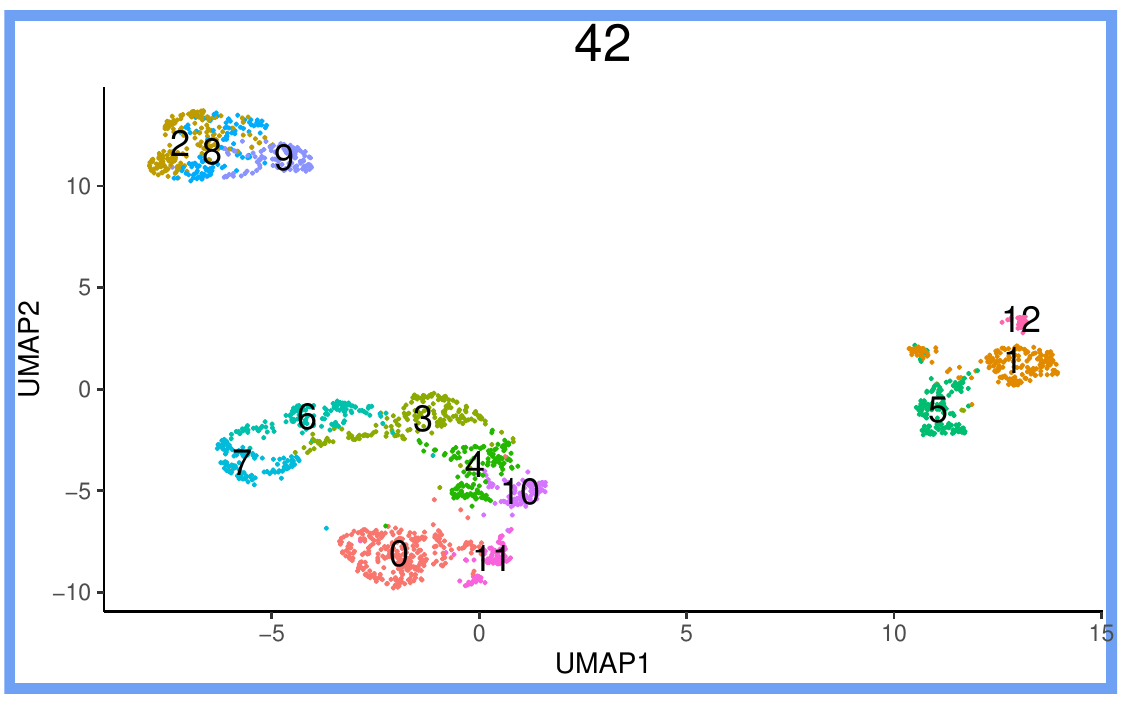
\includegraphics[width=7cm]{2_S1.png}
    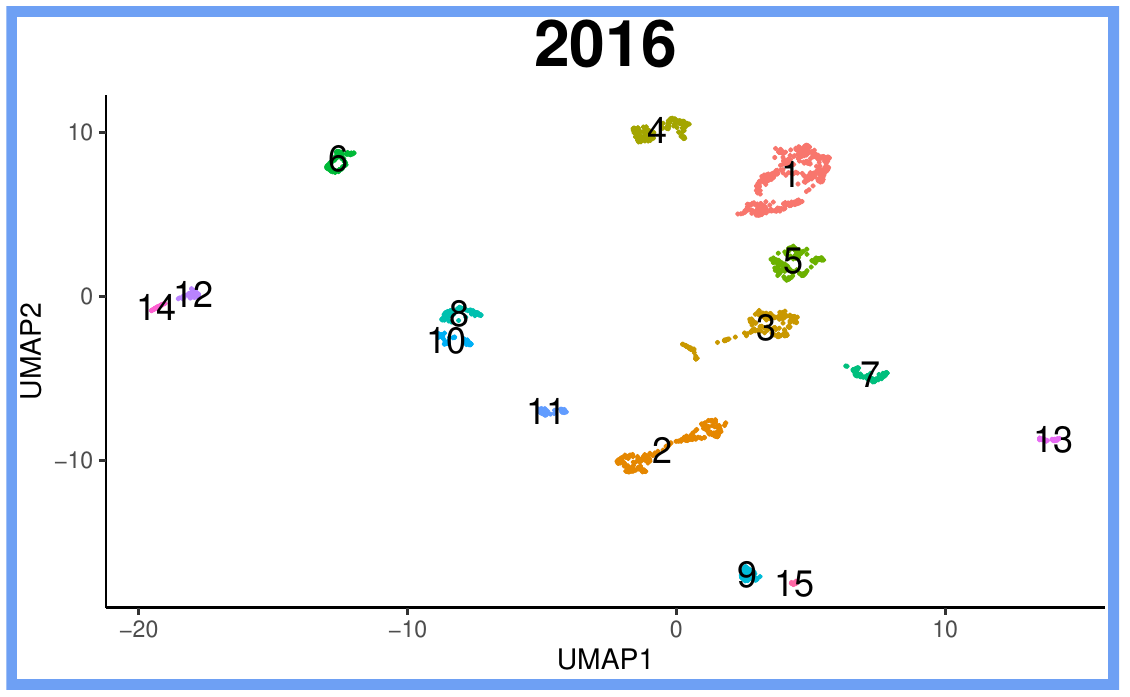
\includegraphics[width=7cm]{2_M1.png}
    \caption{\label{fig:s4-m3-default}Clustering distribution with default parameters for Monocle (left) and Seurat (right). The title indicates the default random seed that is used.}
\end{figure}

If the Cuomo \cite{Cuomo2020} dataset is clustered using the Monocle and Seurat packages with default parameters, significantly different outputs are produced, as it can be observed in Figure \ref{fig:s4-m3-default}. Firstly, there are differences with respect to the dimensionality reduction. The cells are scattered in multiple islands in the Monocle package, whereas Seurat obtains a more compact grouping. Also, the two packages disagree regarding the number of clusters: Seurat outputs 13 clusters, Monocle 15.

The biological interpretation of the data heavily relies on the clusters' structure. Thus, is expected for the discrepancies between the two packages to extend over the marker identification and the biological interpretation. The question we pose is whether the divergence between Monocle and Seurat has technical (such as the implementation of the clustering pipeline) or biological (such as additional pre- or post-processing steps that rely on the sequencing information).

\section{Aligning the results}




